\documentclass{article}
\usepackage{amsmath,amssymb,graphicx,xcolor,tikz,hyperref,booktabs,geometry,listings}
\usepackage{pgfplots}\pgfplotsset{compat=1.18}
\usetikzlibrary{arrows.meta,shadings,patterns,decorations.pathmorphing}
\begin{document}
\section{Hello}Text $\int_0^1 x^2\,dx$, \href{https://example.com}{link}, \textbf{bold} \emph{it}.
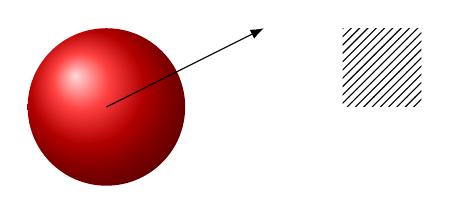
\begin{tikzpicture}\shade[ball color=red] (0,0) circle (1);\draw[-{Latex}] (0,0) -- (2,1);\fill[pattern=north east lines](3,0) rectangle (4,1);\end{tikzpicture}
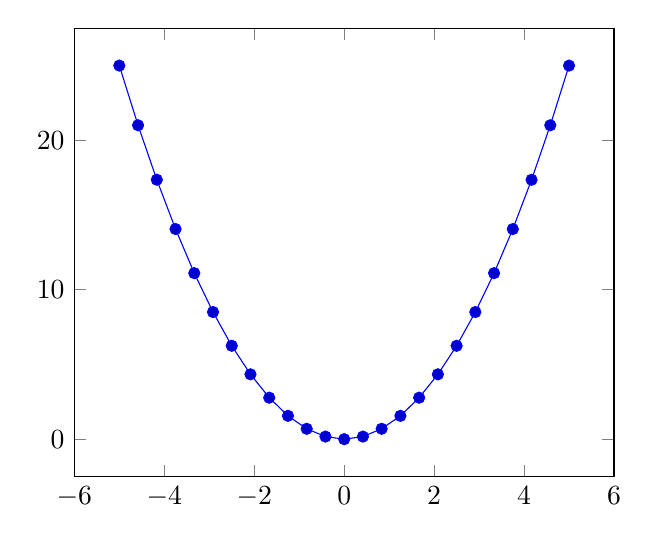
\begin{tikzpicture}\begin{axis}\addplot{x^2};\end{axis}\end{tikzpicture}
\end{document}
